\section{The study of the cost efectiveness of vaccinating only girls, only boys or both}\label{coste_efectividad}

The apparition of the paper of \cite{elbasha2007model} determined the vaccination strategy used in all the countries, that is, the vaccination of young girls before having contact with HPV. This strategy has been fruitful and has prevented infections in girls (by vaccination) and boys (by the herd immunity). However, the men who have sex with men (MSM) is a group where the prevalence of HPV is high and difficult to reduce only vaccinating women, becoming this group a reservoir of the HPV. Also, it does not happen the same with women, that is, women who have sex with women have a very low HPV prevalence.

Considering that one of the current discussions is about the pertinence of vaccinating boys as well, it is possible to simulate different vaccination strategies using the proposed model and compare the results.

Here, we are going to compare three scenarios:

\begin{itemize}
	\item Scenario 1: vaccination of $75\%$ girls before 14 years old,
	\item Scenario 2: vaccination of $75\%$ boys before 14 years old,
	\item Scenario 3: vaccination of $75\%$ girls and boys before 14 years old.
\end{itemize} 

We are not going to consider other possible strategies involving vaccination for older boys and girls because the effectivenes of the vaccine drops in people who have previous contact with HPV \cite{Skufca}. 
%Although, the general drop is high, as we suggested in the Chapter \ref{Australiano}, considering all the possible infections, it does not seem to be as high as the authors say \cite{Skufca}.

It is clear that the more we vaccinate, the less prevalence. Nevertheless, the cost should be also evaluated. Hence, the aim of this simulation is to find out if vaccinating only boys is significantly better than vaccination only girls. Also, if the extra cost of vaccinating boys and girls leads to a substantial reduction of prevalence compared with the vaccination of only boys or only girls. 

In Figures \ref{fig:compara_1_1}, \ref{fig:compara_1_2} and \ref{fig:compara_2_1} we compare graphically pairwise the decline HPV oncogenic and HPV 6/11 infections for the three aforementioned strategies.

\begin{figure}[!]
	\centering
	\begin{tabular}{cc}
		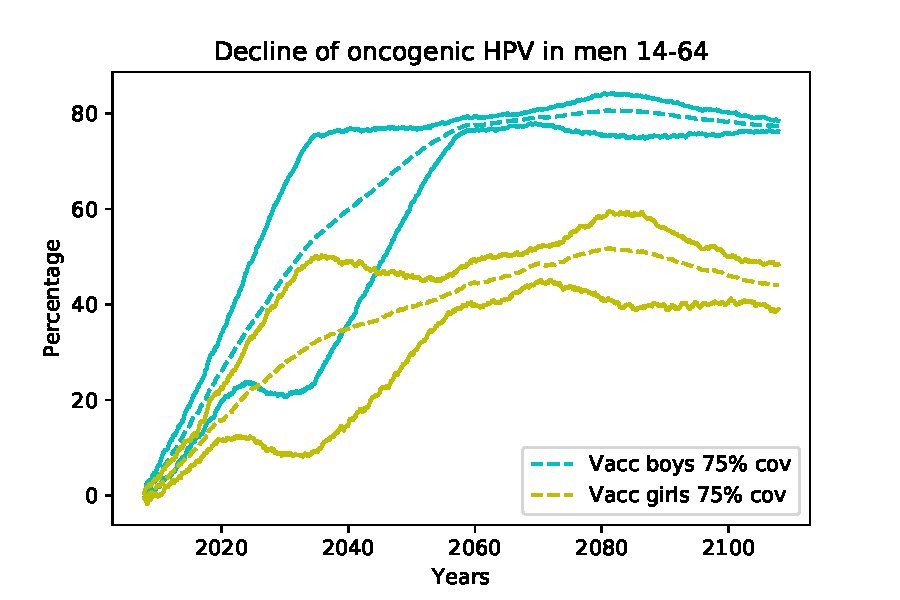
\includegraphics[width=0.5\linewidth]{IMGs/10.-Coste_efectividad/solo_hom_y_solo_muj/onco_hom.pdf}	& 
		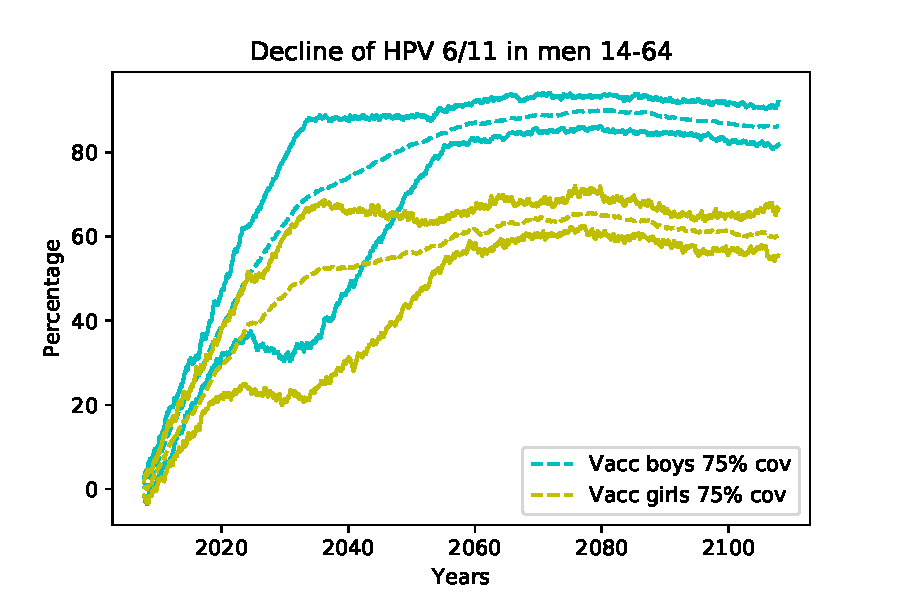
\includegraphics[width=0.5\linewidth]{IMGs/10.-Coste_efectividad/solo_hom_y_solo_muj/verr_hom.pdf}  \\ 
		Decline oncogenic HPV men	& Decline HPV 6/11 men \\ 
		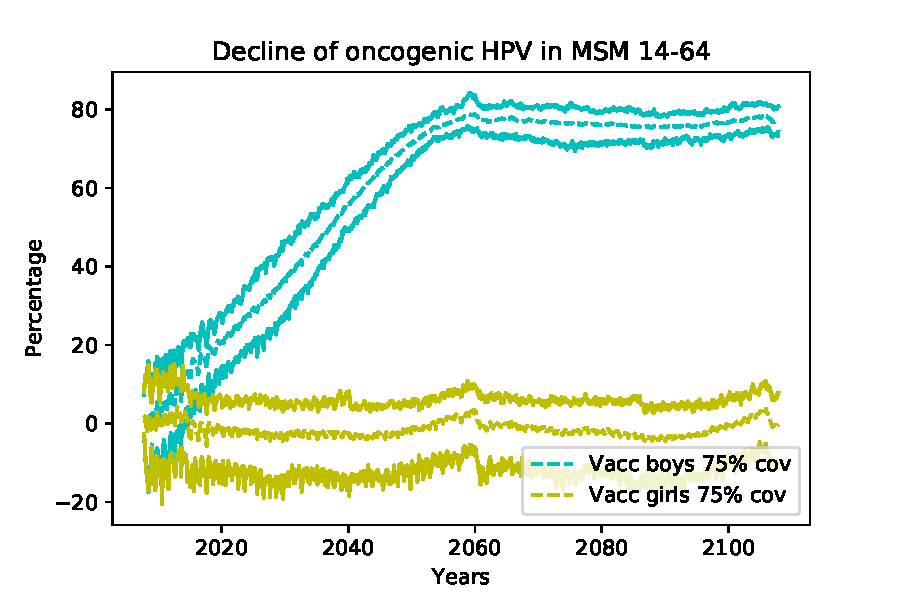
\includegraphics[width=0.5\linewidth]{IMGs/10.-Coste_efectividad/solo_hom_y_solo_muj/onco_MSM.pdf}	& 
		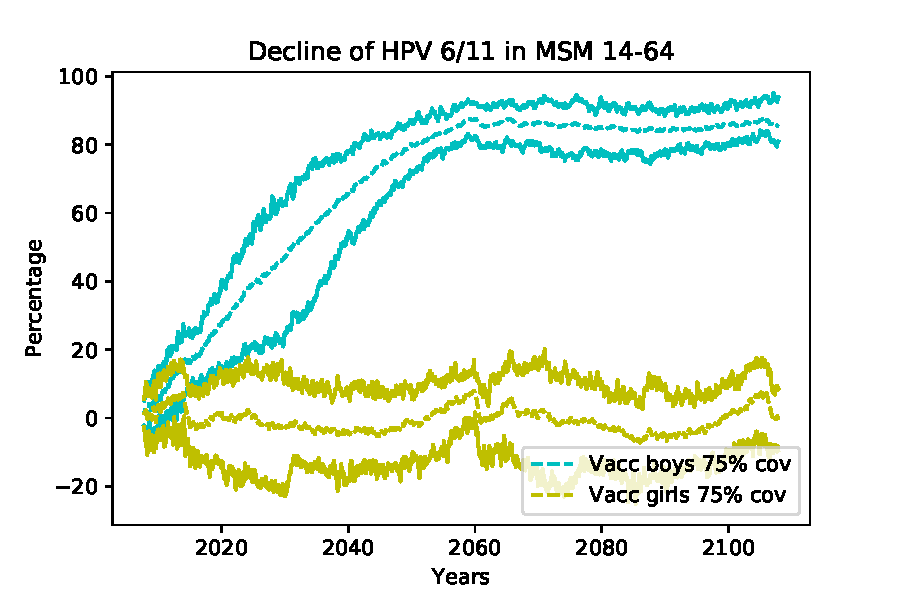
\includegraphics[width=0.5\linewidth]{IMGs/10.-Coste_efectividad/solo_hom_y_solo_muj/verr_MSM.pdf}  \\ 
		Decline oncogenic HPV MSM	& Decline HPV 6/11 MSM \\ 
		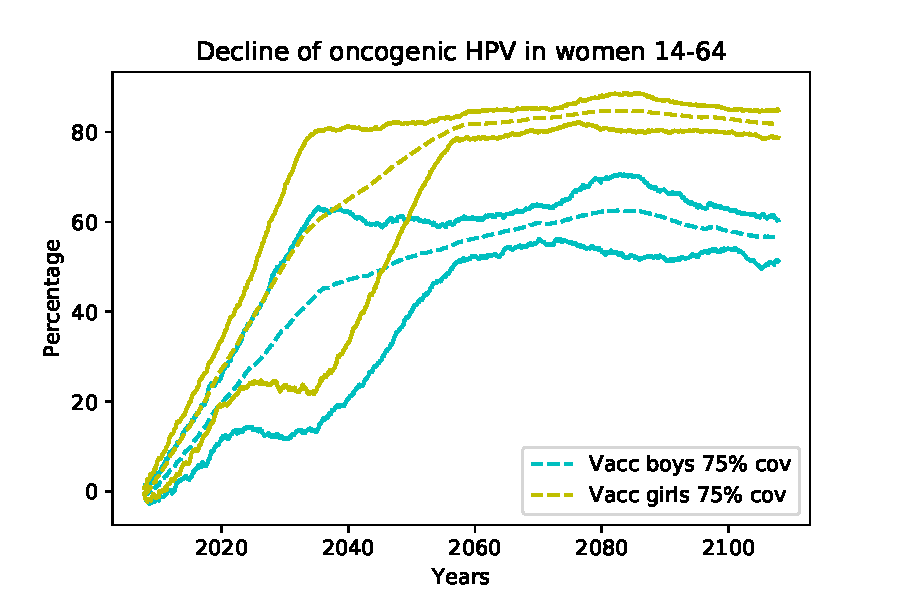
\includegraphics[width=0.5\linewidth]{IMGs/10.-Coste_efectividad/solo_hom_y_solo_muj/onco_muj.pdf}	& 
		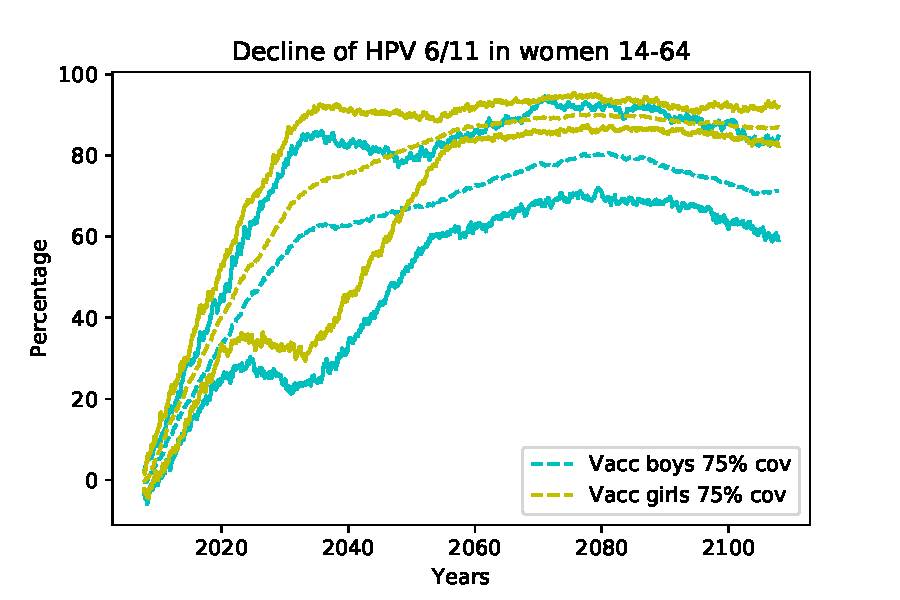
\includegraphics[width=0.5\linewidth]{IMGs/10.-Coste_efectividad/solo_hom_y_solo_muj/verr_muj.pdf}  \\ 
		Decline oncogenic HPV women	& Decline HPV 6/11 women \\ 
	\end{tabular} 
	\caption{Comparative of the decline of HPV between the scenario 1 and 2. MSM benefits in scenario 2 (vaccination of boys). Also, the decline in women is higher in scenario 2 than the decline in men in scenario 1. It seems that the herd immunity effect is greater in scenario 2.}
	\label{fig:compara_1_1}
\end{figure}

Figure \ref{fig:compara_1_1} show a comparison between scenarios 1 and 2, where only girls or only boys are vaccinated. From the economic point of view, both scenarios have a similar cost. Vaccinating boys only (scenario 2) has a direct effect on the decline of HPV infections in MSM, inexistent if we only vaccinate girls (scenario 1). Note that scenario 2 intends to protect the group with higher prevalence, the MSM. 

Now, let us pay attention in the following. The direct protection in both scenarios in the long-run are similar, that is, 

\begin{itemize}
\item in scenario 1 (only vaccinating girls) the average oncogenic HPV decline in girls is $77.4\%-80.6\%$ and in scenario 2 (only vaccinating boys) the average oncogenic HPV decline in boys is $81.8\%-84.8\%$;
\item in scenario 1 (only vaccinating girls) the average HPV 6/11 decline in girls is $85.9\%-90.0\%$ and in scenario 2 (only vaccinating boys) the average oncogenic HPV decline in boys is $86.5\%-90.2\%$.
\end{itemize}

Nevertheless, the cross protection provided by the herd immunity effect is not the same. Only vaccinating girls (scenario 1) gives an average decline of oncogenic HPV in men in the long-run of $43.9\%-51.8\%$ and an average decline of HPV 6/11 of $59.7\%-65.7\%$.

On the other hand, only vaccinating boys (scenario 2) returns an average decline of oncogenic HPV in women in the long-run of $56.4\%-62.6\%$ and an average decline of HPV 6/11 of $70.3\%-80.5\%$, which is much better than scenario 1.

Here, the question that policy makers should answer is, taking into account the high incidence of cervical cancer, is it convenient to change the vaccination strategy vaccinating only men and achieving an average decline of oncogenic HPV in women of $56.4\%-62.6\%$? 

\begin{figure}[!]
	\centering
	\begin{tabular}{cc}
		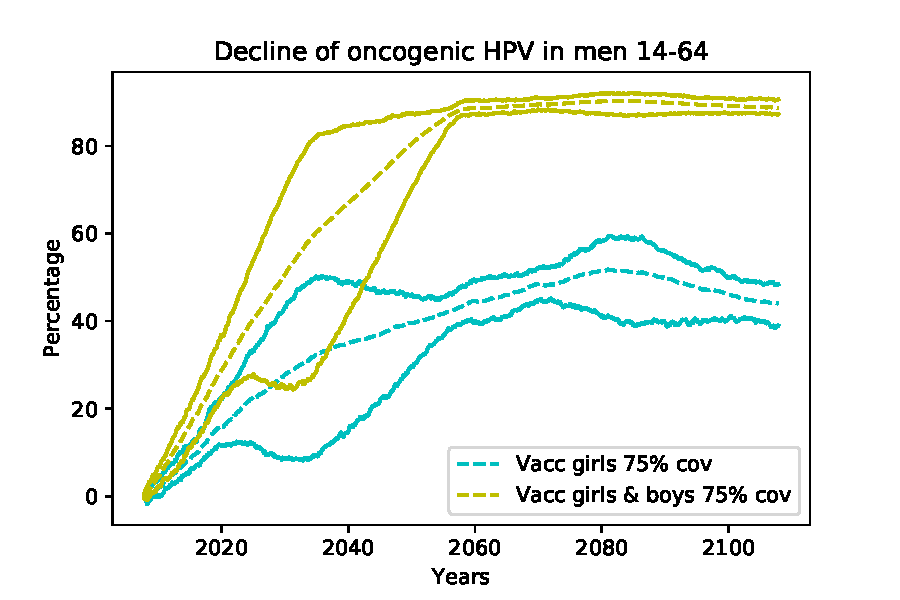
\includegraphics[width=0.5\linewidth]{IMGs/10.-Coste_efectividad/solo_muj_y_ambos/onco_hom.pdf}	& 
		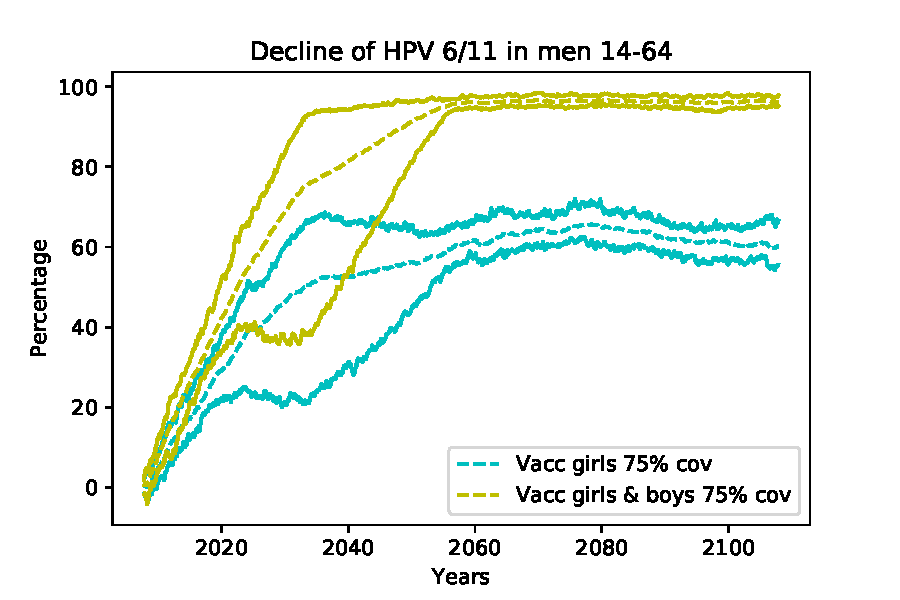
\includegraphics[width=0.5\linewidth]{IMGs/10.-Coste_efectividad/solo_muj_y_ambos/verr_hom.pdf}  \\ 
		Decline oncogenic HPV men	& Decline HPV 6/11 men \\ 
		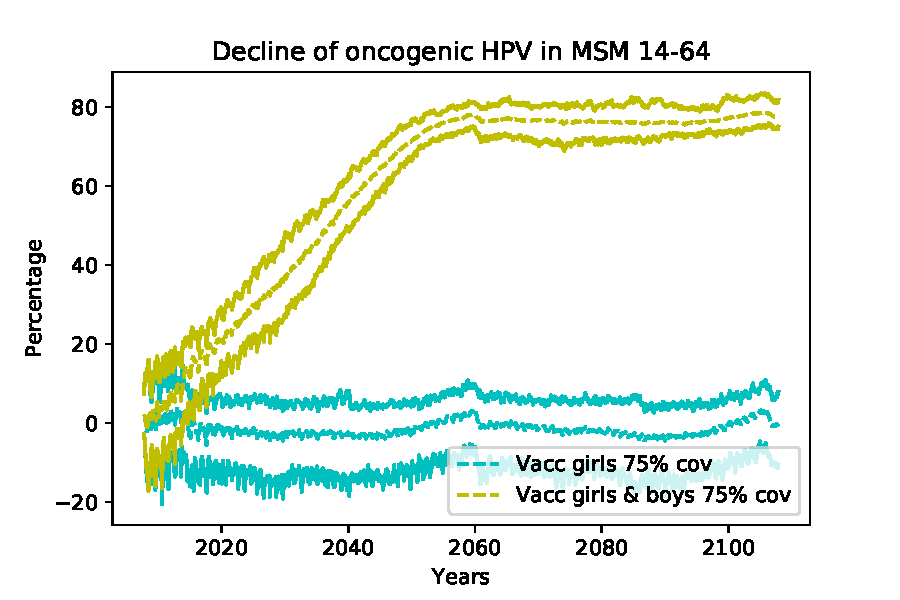
\includegraphics[width=0.5\linewidth]{IMGs/10.-Coste_efectividad/solo_muj_y_ambos/onco_MSM.pdf}	& 
		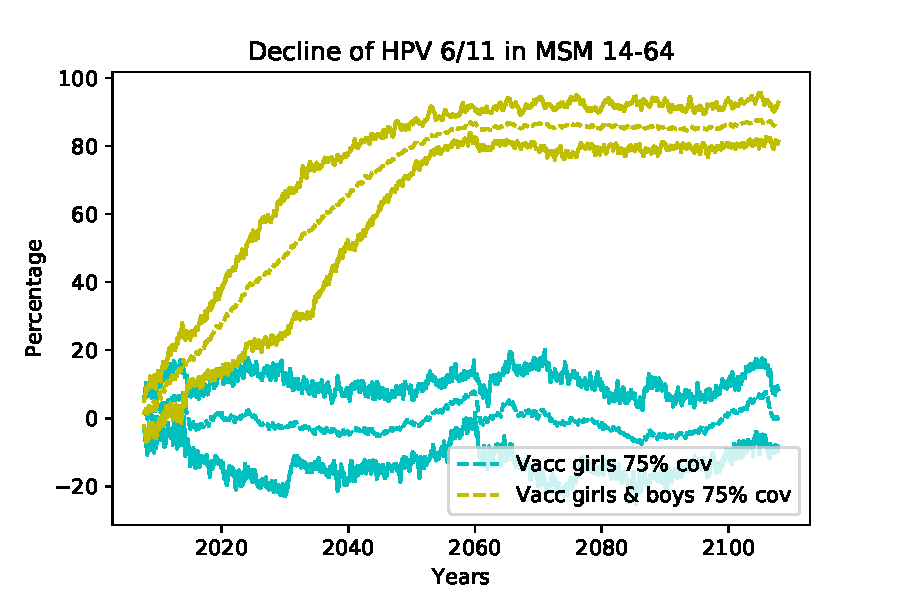
\includegraphics[width=0.5\linewidth]{IMGs/10.-Coste_efectividad/solo_muj_y_ambos/verr_MSM.pdf}  \\ 
		Decline oncogenic HPV MSM	& Decline HPV 6/11 MSM \\ 
		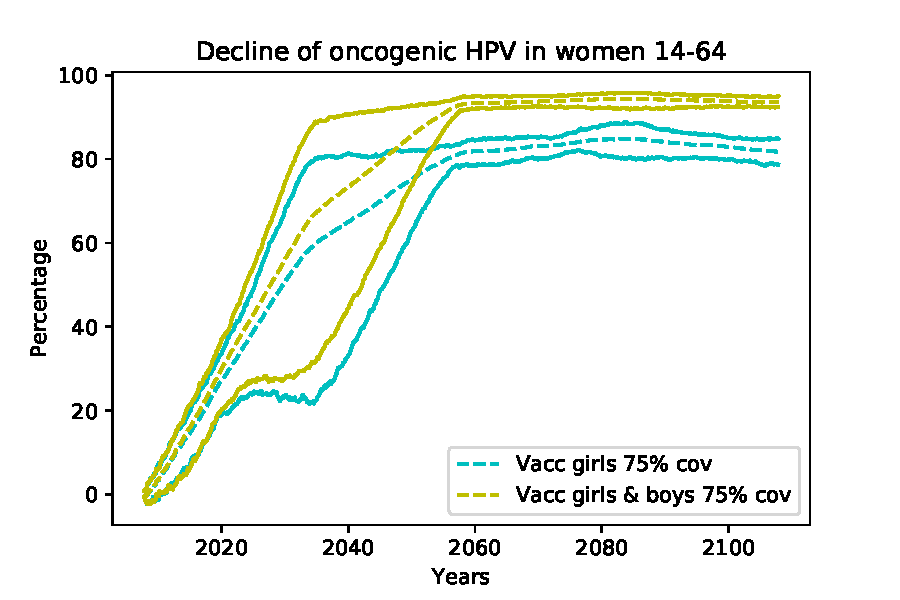
\includegraphics[width=0.5\linewidth]{IMGs/10.-Coste_efectividad/solo_muj_y_ambos/onco_muj.pdf}	& 
		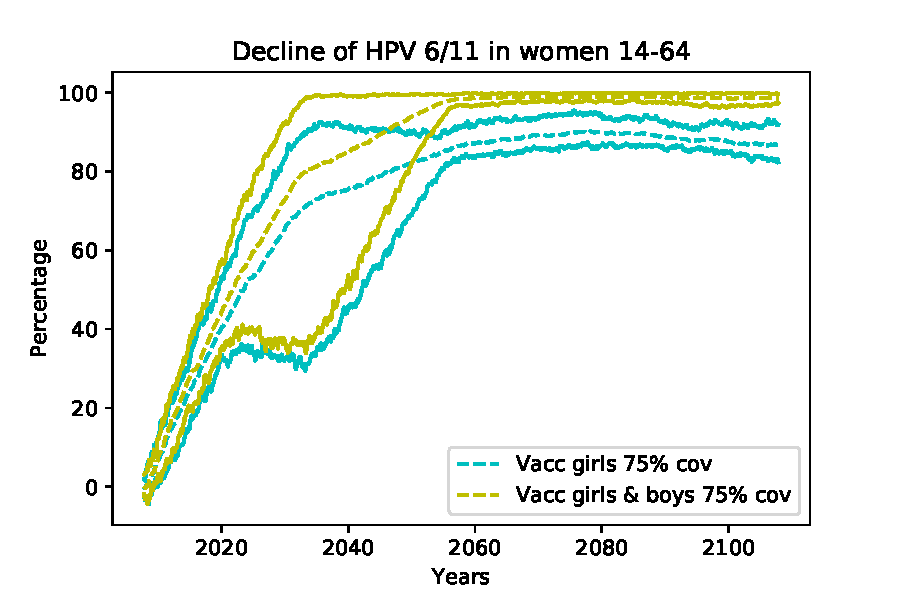
\includegraphics[width=0.5\linewidth]{IMGs/10.-Coste_efectividad/solo_muj_y_ambos/verr_muj.pdf}  \\ 
		Decline oncogenic HPV women	& Decline HPV 6/11 women \\ 
	\end{tabular} 
	\caption{Comparative of the decline of HPV between the scenario 1 and 3. The decline in scenario 3 is higher in all the cases.}
	\label{fig:compara_1_2}
\end{figure}

In Figure \ref{fig:compara_1_2} we can see a comparison between scenarios 1 and 3, where only girls are vaccinated or both boys and girls are vaccinated. From the economic point of view, the vaccination of boys and girls is twice as expensive.

Scenario 3 improves the protection of girls because of the herd immunity of vaccinating boys and the protection of the MSM. Also, there are differences, in average, around $38.4\%-44.7\%$ and $30.8\%-36.5\%$ between the declines of the considered scenarios for oncogenic HPV and HPV 6/11 in men, respectively.

\begin{figure}[!]
	\centering
	\begin{tabular}{cc}
		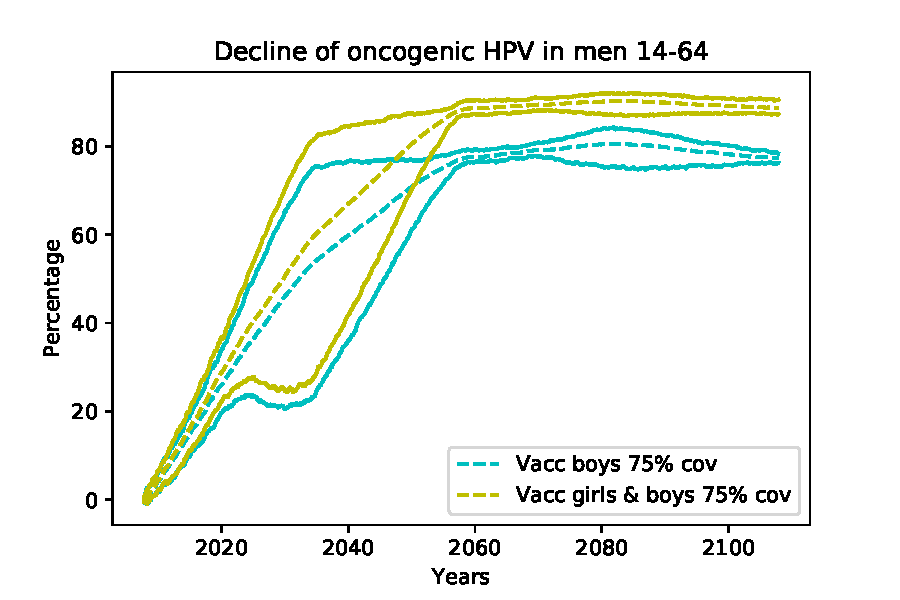
\includegraphics[width=0.5\linewidth]{IMGs/10.-Coste_efectividad/solo_hom_y_ambos/onco_hom.pdf}	& 
		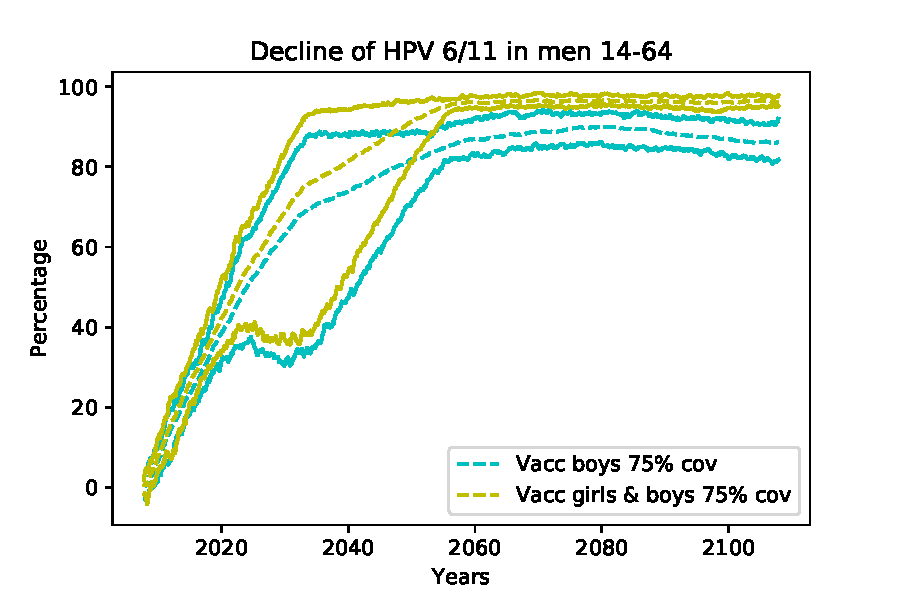
\includegraphics[width=0.5\linewidth]{IMGs/10.-Coste_efectividad/solo_hom_y_ambos/verr_hom.pdf}  \\ 
		Decline oncogenic HPV men	& Decline HPV 6/11 men \\ 
		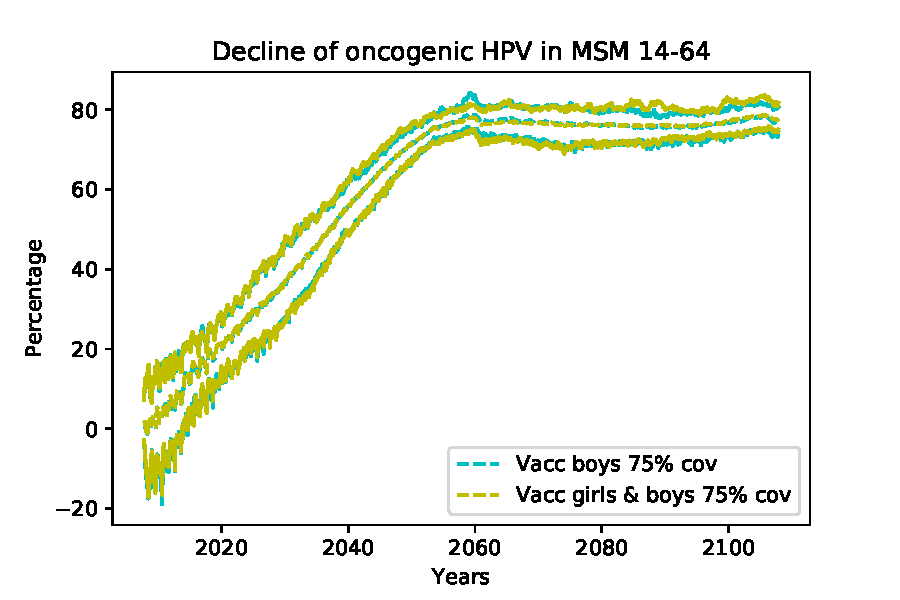
\includegraphics[width=0.5\linewidth]{IMGs/10.-Coste_efectividad/solo_hom_y_ambos/onco_MSM.pdf}	& 
		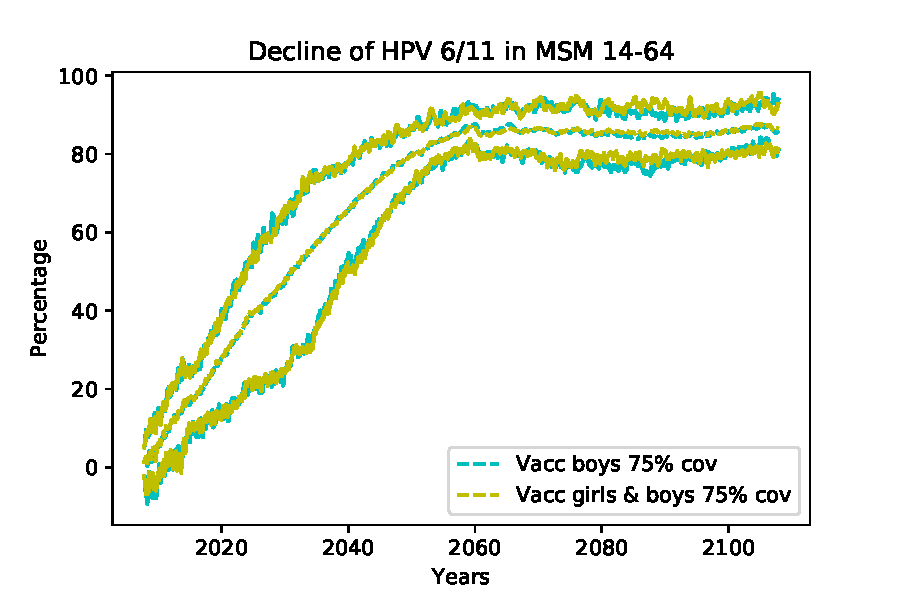
\includegraphics[width=0.5\linewidth]{IMGs/10.-Coste_efectividad/solo_hom_y_ambos/verr_MSM.pdf}  \\ 
		Decline oncogenic HPV MSM	& Decline HPV 6/11 MSM \\ 
		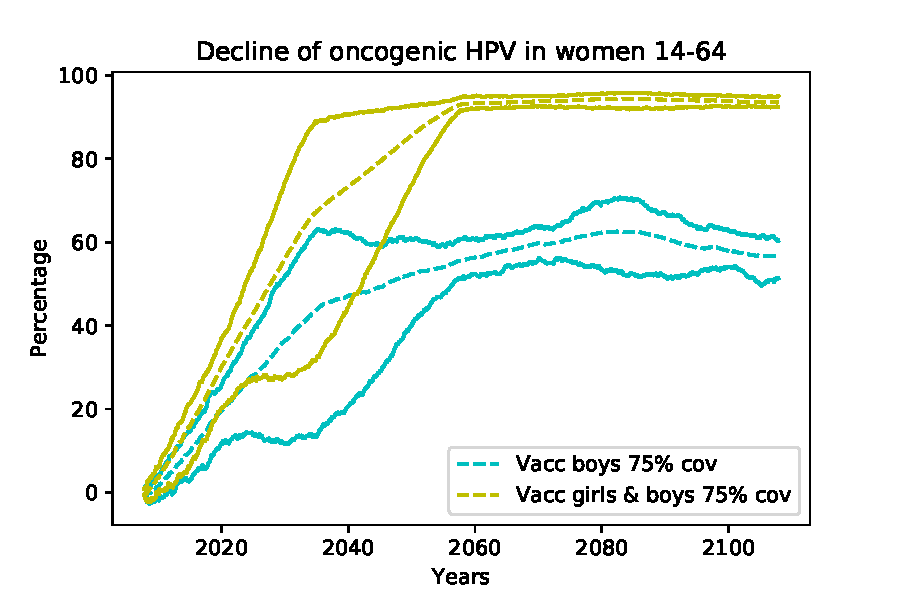
\includegraphics[width=0.5\linewidth]{IMGs/10.-Coste_efectividad/solo_hom_y_ambos/onco_muj.pdf}	& 
		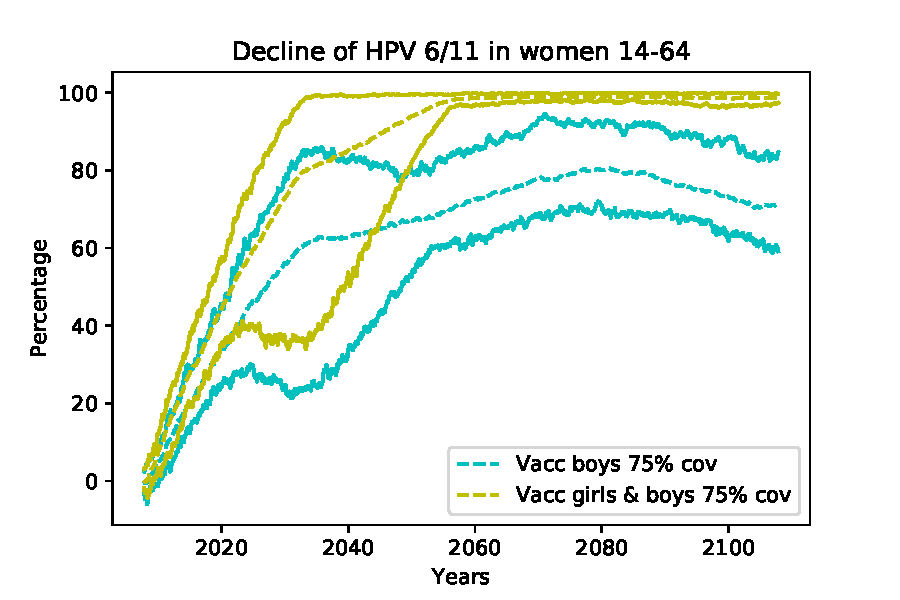
\includegraphics[width=0.5\linewidth]{IMGs/10.-Coste_efectividad/solo_hom_y_ambos/verr_muj.pdf}  \\ 
		Decline oncogenic HPV women	& Decline HPV 6/11 women \\ 
	\end{tabular} 
	\caption{Comparative of the decline of HPV between the scenario 2 and 3. The decline in scenario 3 is slightly higher for men and women, and the same for MSM.}
	\label{fig:compara_2_1}
\end{figure}

Now, in Figure \ref{fig:compara_2_1} there is the graphical comparison between scenarios 2 and 3, where only boys are vaccinated or both boys and girls are vaccinated. As we mentioned before, economically the vaccination of boys and girls is twice as expensive.

Scenario 3 improves the protection of boys because of the herd immunity of vaccinating girls. Also, there are differences, in average, around $31.8\%-37.0\%$ and $18.5\%-28.4\%$ between the declines of the considered scenarios for oncogenic HPV and HPV 6/11 in women, respectively. These declines are less than the corresponding ones from the comparison between scenario 1 and 3.

Thus, the best strategy is to vaccinate boys and girls (scenario 3), but it is the more expensive. Between scenario 1 and 2, scenario 2 (only vaccination of boys) achieves better levels of decline than scenario 1. However, scenario 2 has a main drawback, and it is that the levels of decline, in average, for oncogenic HPV in women are $56.4\%-62.6\%$ and it may be considered as insufficient in a situation where the cervical cancer is the most threaten pathology due to HPV, being a direct consequence of oncogenic HPV infections.     



